%% -*- coding:utf-8 -*-
\chapter{Monads}

Monads are very important for pure functional programming languages
such as Haskell. We will start with formal mathematical definition and
will continue with programming languages examples later.


\section{Monoidal category}

\begin{definition}[Monoidal category]
\label{def:monoidal_category}
A category $\cat{C}$ is called \textit{monoidal category} if it is
equipped with a \mynameref{def:monoid} structure i.e. there are
\begin{itemize}
\item \mynameref{def:bifunctor} $\otimes: \cat{C} \times \cat{C} \tof
  \cat{C}$ called \textit{monoidal product} \index{Monoidal
    product!definition} 
\item an \mynameref{def:object} $id$ called unit object or identity object
\end{itemize}

The elements should satisfy (up to \mynameref{def:isomorphism}) several conditions:
associativity: 
\begin{equation}
A \otimes \left( B \otimes C \right) \cong_\alpha
  \left( A \otimes B \right) \otimes C,
\nonumber
\end{equation}
where $\alpha$ is called associator. \index{Associator!definition}
$id$ can be treated as left and right identity: 
\begin{eqnarray}
id \otimes A \cong_\lambda A, 
\nonumber \\
A \otimes id \cong_\rho A,
\nonumber
\end{eqnarray}
where $\lambda, \rho$ are called as left and right unitors respectively. \index{Left unitor!definition} \index{Right unitor!definition}
\end{definition}


\begin{definition}[Strict monoidal category]
\label{def:strict_monoidal_category}
\index{Associator}
A \mynameref{def:monoidal_category} $\cat{C}$ is said to be strict if the
associator, left 
unitor and right unitors are all identity morphisms i.e.
\[
\alpha = \lambda = \rho = \idm{C}.
\]
\index{Left unitor} \index{Right unitor}
\end{definition}

\begin{remark}[Monoidal product]
\label{rem:monoidal_product}
The monoidal product is a binary operation that specifies the exact
monoidal structure. Often it is called as \textit{tensor product} but
we will avoid the naming because it is not always the same as the
\mynameref{def:tensor_product} as it is introduced for
\mynameref{def:hilbert_space}s  
\end{remark}

\begin{definition}[Tensor product]
  \label{def:tensor_product}
  TBD
\end{definition}


\section{Category of endofunctors}

The \mynameref{ex:fun_category} is an example of a category. We can
apply additional limitation and consider only
\mynameref{def:endofunctor}s i.e. we will look at the category
$[\cat{C}, \cat{C}]$ - category of functors from category $\cat{C}$ to
the same category. One of the most popular math definition of a monad
is the following: 
``All told, a monad in X is just a monoid in the category of
endofunctors of X''\cite{bib:maclane71}.
Later we will give an explanation for that one.

\begin{definition}[Monad]
  \label{def:monad}
  The monad $M$ is an \mynameref{def:endofunctor} with 2
  \mynameref{def:nt}s:
  \begin{enumerate}
  \item $\eta: \idf{C} \tont M$
  \item $\mu: M \circ M \tont M$
  \end{enumerate}
  where $\idf{C}$ is \mynameref{def:idfunctor}.

  The $\eta, \mu$ should satisfy the following conditions:
  \begin{eqnarray}
    \mu \circ M \mu = \mu \circ \mu M, 
    \nonumber \\
    \mu \circ M \eta = \mu \circ \eta M = \idnt{M},
    \label{eq:monad}
  \end{eqnarray}
  where $M \mu, M \eta$ - \mynameref{def:rw}s, $\mu M, \eta M$ -
  \mynameref{def:lw}s, $\idnt{M}$ - \mynameref{def:idnt} for $M$.
  \mynameref{def:vertical_composition} is used in the equations.

  The monad will be denoted later as $\left<M, \mu, \eta\right>$.
\end{definition}

Lets look at the requirements \eqref{eq:monad} more closely. 
First of
all rewrite it with \eqref{eq:lw} and \eqref{eq:rw} as follows
\begin{eqnarray}
  \mu \circ \left( \idnt{M} \star \mu \right) = 
  \mu \circ \left( \mu \star \idnt{M} \right), 
  \nonumber \\
  \mu \circ \left( \idnt{M} \star \eta \right) = 
  \mu \circ \left( \eta \star \idnt{M} \right) = \idnt{M}.
  \label{eq:monad_p1}
\end{eqnarray}
The first equation can be represented as a
\mynameref{def:commutative_diagram} (see \cref{fig:monad_monoid1})
\begin{figure}
  \centering
  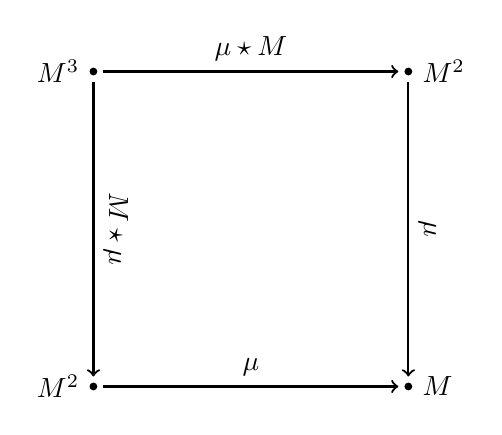
\begin{tikzpicture}[ele/.style={fill=black,circle,minimum
        width=.8pt,inner sep=1pt},every fit/.style={ellipse,draw,inner
        sep=-2pt}]

    % the texts
    
    \node[ele,label=left:$M^3$] (m3) at (0,4) {};    
    \node[ele,label=left:$M^2$] (m21) at (0,0) {};    
    \node[ele,label=right:$M^2$] (m22) at (4,4) {};
    \node[ele,label=right:$M$] (m) at (4,0) {};

    \draw[->,thick,shorten <=2pt,shorten >=2pt] (m3) to
    node[sloped,above]{$\idnt{M} \star \mu$} (m21);
    \draw[->,thick,shorten <=2pt,shorten >=2] (m3) to
    node[sloped,above]{$\mu \star \idnt{M}$} (m22); 
    \draw[->,thick,shorten <=2pt,shorten >=2] (m21) to
    node[sloped,above]{$\mu$} (m); 
    \draw[->,thick,shorten <=2pt,shorten >=2] (m22) to
    node[sloped,above]{$\mu$} (m); 
  \end{tikzpicture}
  \caption{Monad as monoid in the category of endofunctors.}
  \label{fig:monad_monoid1}
\end{figure}
Let look how the first equation acts on $M^3 = M \circ M \circ M$:
\begin{eqnarray}
\left( \idnt{M} \star \mu \right) \left[ M \circ M \circ M
\right] = 
\left( \idnt{M} \star \mu \right) \left[ M \circ \left( M \circ M \right)
\right] = 
\nonumber \\
= M \circ \left(M \otimes M\right), 
\nonumber
\end{eqnarray}
where properties \mynameref{def:horizontal_composition} and the
following equations were used:
\[
\mu \left(M \circ M\right) = M \otimes M \in [\cat{C}, \cat{C}]
\]
and
\[
\idnt{M}\left(M\right) = M.
\]
Therefore
\begin{eqnarray}
\mu \circ \left( \idnt{M} \star \mu \right) \left[ M \circ M \circ M
\right] = 
\nonumber \\
=
\mu \left[M \circ \left(M \otimes M\right)\right] = 
M \otimes \left(M \otimes M\right).
\label{eq:monad_p1_1_left}
\end{eqnarray}
The second part of the first equation \eqref{eq:monad_p1} gives us
\begin{eqnarray}
\mu \left( \mu \star \idnt{M} \right) \left[ M \circ M \circ M
\right] = 
\nonumber \\
=
\mu \left( \mu \star \idnt{M} \right) \left[ \left(M \circ M\right)
  \circ M \right] = 
\nonumber \\
= \mu \left[\left(M \otimes M\right) \circ M \right] = 
\left(M \otimes M\right) \otimes M. 
\label{eq:monad_p1_1_right}
\end{eqnarray}
Combining \eqref{eq:monad_p1_1_left} and \eqref{eq:monad_p1_1_right}
one can get
\[
M \otimes \left(M \otimes M\right) = 
\left(M \otimes M\right) \otimes M
\]
i.e. the first equation \eqref{eq:monad_p1} provides the associativity
(the first property that each \mynameref{def:monoid} should satisfy). 

There should be an identity element for each \mynameref{def:monoid}.
Lets show that the second equation of  \eqref{eq:monad_p1} provides us
the required element. Lets $U =
\eta\left(\idf{C}\right)$. 
We want to show that 
\begin{equation}
U \otimes M = M \otimes U = M, 
\nonumber
\end{equation}
that is exactly required as identity presence in the
\mynameref{def:monoid} definition.
Consider the action of the left part of second equation
\eqref{eq:monad_p1} on $M = M \circ \idf{C}$:
\begin{eqnarray}
\mu \circ \left( \idnt{M} \star \eta \right) \left[M \circ \idf{C}\right] = 
\nonumber \\
=
\mu \left[M \circ U\right] = M \otimes U
\nonumber
\end{eqnarray}
For the middle part of  of second equation
\eqref{eq:monad_p1}
\begin{eqnarray}
\mu \circ \left( \eta \star \idnt{M} \right) \left[M\right] = 
\mu \circ \left( \eta \star \idnt{M} \right) \left[\idf{C} \circ M\right] = 
\nonumber \\
=
\mu \left[U \circ M\right] = U \otimes M.
\nonumber
\end{eqnarray}
Thus
finally
\[
M \otimes U = U \otimes M = M
\]
that finals the proof of monoidal structure.

\section{Kleisli category. Monads in programming languages}

\begin{definition}[Kleisli category]
\label{def:kleisli_category}
Let $\cat{C}$ is a category, $M$ is an \mynameref{def:endofunctor} and
$\left<M, \mu, \eta\right>$ is a \mynameref{def:monad}. Then we can
construct a new category $\cat{C_M}$ that is called as \textit{Kleisli
  category} as follows:
\begin{eqnarray}
\catob{C_M} = \catob{C},
\nonumber \\
\hom_{\cat{C_M}}\left(a, b\right) = 
\hom_{\cat{C}}\left(a, M(b)\right)
\nonumber
\end{eqnarray}
i.e. objects of categories $\cat{C}$ and $\cat{C_M}$ are the same but
morphisms from $\cat{C_M}$ form a subset of morphisms $\cat{C_M}$:
$\cathom{C_M} \subset \cathom{C}$.
\end{definition}

\subsection{Programming languages}
\mynameref{def:kleisli_category} widely spread in programming
especially it provides good description for different types of
computations, for instance \cite{bib:Moggi91, bib:milewski2018category} 
\begin{itemize}
\item \textbf{Partiality} i.e. then a function not defined for each input, for
  instance the following expression is undefined (or partially
  defined) for $x = 0$: $f(x) = \frac{1}{x}$
\item \textbf{Non-Determinism} i.e. then multiply output are possible
\item \textbf{Side-effects} i.e. TBD
\item \textbf{Exception} i.e. TBD
\item \textbf{Continuation} i.e. TBD
\item \textbf{Interactive input} i.e. TBD
\item \textbf{Interactive output} i.e. TBD
\end{itemize}

TBD

\section{Examples}

\subsection{Programming languages}

\subsubsection{Haskell}

\begin{example}[Monad][\textbf{Hask}]
\label{ex:monad_haskell}
In Haskell monad can be defined from \mynameref{ex:functor_haskell} as follows 
\footnote{real definition is quite different from the presented one}
\begin{minted}{haskell}
    class Functor m => Monad m where
        return :: a -> m a
        (>>=)  :: m a -> (a -> m b) -> m b
\end{minted} 

To show how this one can be get we can start from a definition that is
similar to the math definition:
\begin{minted}{haskell}
    class Functor m => Monad m where
        return :: a -> m a
        join  :: m (m a) -> m a
\end{minted} 
where \mintinline{haskell}{return} can be treated as $\eta$ and 
\mintinline{haskell}{join} as $\mu$. In the case the bind operator 
\mintinline{haskell}{>>=} can be implemented as follows
\begin{minted}{haskell}
(>>=)  :: m a -> (a -> m b) -> m b
ma >>= f = join ( f ma )
\end{minted} 

\end{example}

\begin{example}[Maybe monad][\textbf{Hask}]
\label{ex:maybe_monad_haskell}
Consider the monad definition that is most close to math definition
first:
\begin{minted}{haskell}
    class Functor m => Monad m where
        return :: a -> m a
        join  :: m (m a) -> m a
\end{minted} 
the Maybe monad can be implemented as follows
\begin{minted}{haskell}
  instance Monad Maybe where
    return = Just
    join Just( Just x) = Just x
    join _ = Nothing
\end{minted} 

\end{example}
TBD

\subsubsection{C++}

TBD

\subsubsection{Scala}

\begin{example}[Monad][\textbf{Scala}]
The monad concept is Scala is more close to formal math definition for
\mynameref{def:monad}. It can be defined as follows 
\footnote{real definition is quite different from the presented one}
\label{ex:monad_scala}
\begin{minted}{scala}
trait M[A] {
  def flatMap[B](f: A => M[B]): M[B]
}
  
def unit[A](x: A): M[A]
\end{minted} 
I.e. \mintinline{scala}{flatMap} can be considered as $\mu$ and
\mintinline{scala}{unit} as $\eta$. 
\end{example}

TBD

\subsection{Quantum mechanics}

The tensor product in quantum mechanics is used for
representing a system that consists of multiple systems. For instance
if we have an interaction between an 2 level atom ($a$ is excited
state $b$ as a ground state) and one mode light then the
atom has its own Hilber space $\mathcal{H}_{at}$ with $\ket{a}$ and
$\ket{b}$ as basis 
vectors.  Light also has its own Hilber space $\mathcal{H}_f$ with Fock state
$\{\ket{n}\}$ as the basis.
\footnote{
  Really the $\mathcal{H}_f$ is infinite dimensional Hilber space and
  seems to be out of our assumption about \textbf{FdHilb} category as
  a collection of finite dimensional Hilber spaces only.
}
The result system that describes both atom
and light is represented as the tensor product $\mathcal{H}_{at}
\otimes \mathcal{H}_f$.

The morphisms of \textbf{FdHilb} category have a connection with
\mynameref{def:tensor_product}. Consider the so called Hilbert-Schmidt
correspondence for finite dimensional Hilbert spaces i.e. for given
$\mathcal{A}$ and $\mathcal{B}$ there is a natural isomorphism between
the tensor product and linear maps (aka morphisms) between
$\mathcal{A}$ and $\mathcal{B}$:
\[
\mathcal{A}^\ast \otimes \mathcal{B} \cong \hom(\mathcal{A}, \mathcal{B})
\]
where $\mathcal{A}^\ast$ - \mynameref{def:dual_space}.


TBD
